% ###########################################################
% ###########################################################
\ifFIGS
\begin{figure*}[!ht]
  \tikzexternalenable
    \tikzsetnextfilename{comorbidB}
  \vspace{-5pt}

\def\DATA{../../data_latest}
\iftikzX
\input{Figures/figClass1Y3_}
\else
  \includegraphics[width=0.8\textwidth]{Figures/External/comorbidB}
  \fi
  \vspace{-5pt}
  
  \captionN{\textbf{Details of Co-morbidity Patterns (at age $<3$ years)} for immunologic (panel A), respiratory (panel B), infections (panel C),  and disorders with similar pathobiology manifesting opposing association with autism (panel D).}\label{EXT-fig4}
    \vspace{-5pt}

\end{figure*}
\else
\refstepcounter{figure}\label{EXT-fig4}
\fi
%###########################################################
%###########################################################
% % ###########################################################
\ifFIGS
\begin{figure}[!ht]
  \tikzexternalenable
    \tikzsetnextfilename{comorbidC}

  \def\DATA{../../data_revision}

\iftikzX
\input{Figures/figClass5Y3.tex}
\else
  \includegraphics[width=0.9\textwidth]{Figures/External/comorbidC}
  \fi

  \vspace{-0pt}
  
  \captionN{\textbf{Co-morbidity Patterns}  for mental disorders, vaccinations and health-service encounters.}\label{EXT-figvv1}
\end{figure}%##########################################################
\else
\refstepcounter{figure}\label{EXT-figvv1}
\fi
% % % ###########################################################%
%###########################################################
%###############################################
%###########################################################
\ifFIGS
\begin{figure*}[!ht]
  \tikzexternalenable
    \tikzsetnextfilename{nopsych}
  \centering  
  \vspace{-10pt}
  
  \def\DATA{../../data_latest}
  \iftikzX
\input{Figures/figpred1nop_}
\else
  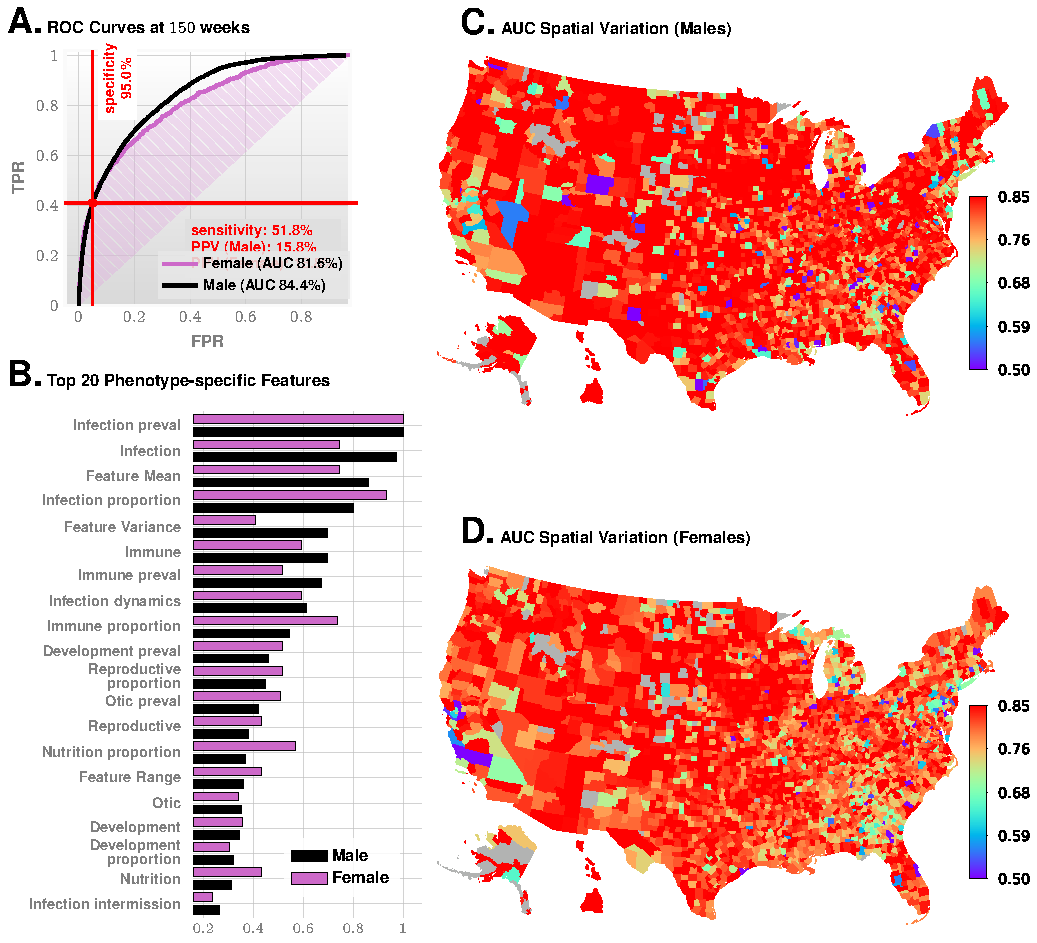
\includegraphics[width=0.95\textwidth]{Figures/External/nopsych}
  \fi 
     \vspace{-5pt}

     \captionN{Predictive Performance without psychiatric codes (ICD9 290 - 319)  and codes for health status and services (ICD9 V0-V91)  included. As shown, the performance is comparable at 150 weeks, with the AUC for females marginally lower (compare with Fig.~\ref{main-fig1} in the main text). The feature importances also are similar, with infectious diseases inferred to have the most importance (or weight) in the pipeline, which is also the case once we add psychiatric phenotypes, and codes for health services in our analysis. As shown in  SI-Fig.~\ref{EXT-figvv1}A, the psychiatric codes all increase risk, and the vaccination codes (See  SI-Fig.~\ref{EXT-figvv1}B) all decrease risk when those codes are included. This is why an alternate analysis was carried out to make sure that we are not picking up on psychiatric codes alone. Note in particular that the sensitivity/specificity point highlighted in panel A above is identical after adding the codes. This suggests that our predictive performance arises from patterns learned from co-morbidities, which are not just neuropsychiatric in nature.}\label{EXT-fig1nop}
\end{figure*}
\else
\refstepcounter{figure}\label{EXT-fig1nop}
\fi
% %###########################################################
